\chapter{REVISÃO BIBLIOGRÁFICA}

% Climatologia observacional do atlântico

% Dinamica do acoplamento no atlantico tropical

% Viés dos modelos acoplados

%\section{Descrição observacional da interação oceano-atmosfera sobre o Atlântico tropical}
\section{Ciclo anual climatológico observado no Atlântico tropical}

A Figura~\ref{fig:oisst_act_clim} mostra as médias mensais da temperatura da superfície do mar média entre 16W-4E e 4S-4N, região afetada pela língua fria do Atlântico, obtidas do produto observacional NOAA OISST V2 para o período entre janeiro de 1982 e dezembro de 2013, com os valores para os 32 anos superpostos mês-a-mês. Os valores estão replicados de modo que o ciclo anual se apresenta com uma repetição, permitindo visualização contínua da variação anual em qualquer fase. A linha cinza que conecta meses adjacentes representa a média climatológica mensal fornecendo, portanto, o ciclo anual climatológico.

\begin{figure}[h!]
\centering
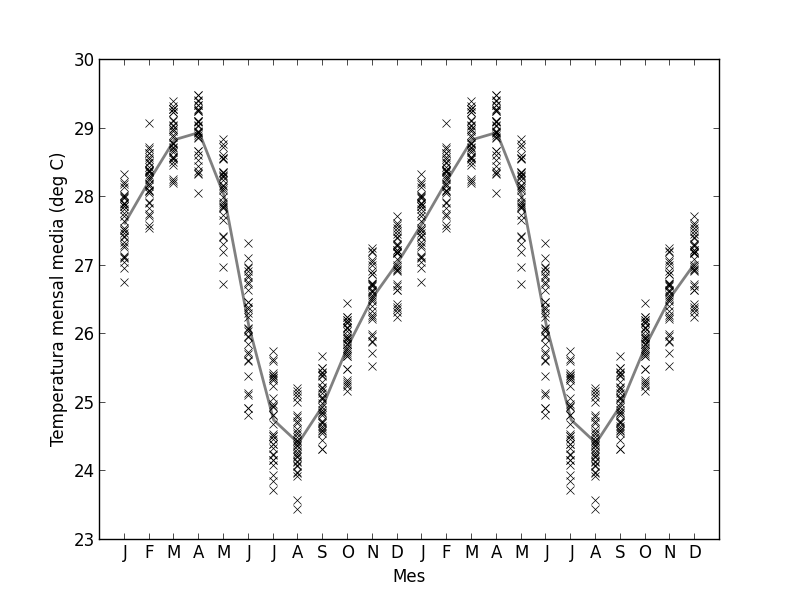
\includegraphics[width=11cm]{figuras/OISST_AtlanticColdTongue.png}
\caption{Médias mensais da temperatura da superfície do mar, média entre $16\,^{\circ}\mathrm{W}$, $4\,^{\circ}\mathrm{E}$ e $4\,^{\circ}\mathrm{S}$, $4\,^{\circ}\mathrm{N}$, referentes ao período entre janeiro de 1982 e dezembro de 2013 do produto NOAA OISST V2.}
\label{fig:oisst_act_clim}
\end{figure}

Pela Figura~\ref{fig:oisst_act_clim} constata-se uma assimetria temporal no ciclo anual, com o resfriamento ocorrendo de forma mais intensa e durando 4 meses, enquanto o aquecimento ocorre durante os 8 meses restantes. \cite{Mitchell/1992}, ao descrever os mecanismos do ciclo anual climatológico da convecção, de TSM e de radiação emitida em onda longa observados na faixa tropical, notando que a maior assimetria entre os hemisférios ocorre em setembro, com máxima penetração dos alíseos de Sul no hemisfério Norte, e quando a língua fria é mais intensa. Para os autores, a língua fria ocorre como consequência da ressurgência equatorial induzida pela tensão superficial do vento de leste que ocorre por causa da convecção sobre as águas mais quentes situadas a oeste. Os autores defendem que que o vento meridional associado às monções sobre os continentes e à ZCIT são instrumentais na efetivação do acoplamento entre atmosfera e oceano e que este acoplamento, por sua vez, é responsável pela proeminência do ciclo anual no setor oeste do cinturão tropical.




%\cite{Mitchell/1992} descrevem o ciclo anual climatológico da convecção e da temperatura da superfície do mar nos trópicos. Para a região do Atlântico, os autores relatam que o ciclo anual, determinado pela marcha do Sol, é o padrão de variabilidade dominante. %variaveis para diagnostico: ROLE, TSM, precipitação, vento.
%\cite{Curtis/1995}, por sua vez, verificam que, durante eventos quentes no Pacífico, 

% figura no formato PDF
% http://stackoverflow.com/questions/8827016/matplotlib-savefig-in-jpeg-format





\subsection{Variabilidade do Atlântico tropical}

\section{Acoplamento oceano-atmosfera no Atlântico tropical: resultados de modelos}